\chapter{Thực nghiệm và đánh giá}
\label{chap:exp}

Chương này lần lượt trả lời ba câu hỏi CH1--CH3 nêu ở mục~\ref{sec:questions}: Thí nghiệm 1 cho CH1, Thí nghiệm 2 cho CH2
và Thí nghiệm 3 cho CH3. Thí nghiệm 3 là trọng tâm vì đo trực tiếp việc thay mặt nạ YOLO bằng bao lồi trực giao.
Chất lượng được đo trên 100 ảnh giao thông Việt Nam có nhãn, với YOLO11-l được chọn ở bước so sánh sơ bộ (mục~\ref{sec:model_select}).
Video không có nhãn nên chỉ dùng để minh hoạ và đo thời gian.

% =====================================================================
\section{Dữ liệu}
\label{sec:data}

Nguồn là bộ \emph{Vietnam Traffic Vehicle Detection} trên Roboflow Universe \cite{roboflowvn} (giấy phép CC BY 4.0):
756 ảnh (601 huấn luyện, 126 kiểm định, 29 kiểm tra), được đưa về kích thước $640\times640$.
Đồ án sử dụng bốn lớp \texttt{car}, \texttt{truck}, \texttt{bus}, \texttt{motorcycle}. Ảnh được trích từ nhiều video camera giao thông.

Bộ đánh giá 100 ảnh được xây dựng từ bộ nguồn theo quy trình:
\begin{enumerate}
  \item Chỉ giữ ảnh mà \emph{mọi} nhãn phương tiện đều là polygon, tức đa giác mô tả đường viền xe; loại ảnh có nhãn chỉ ở dạng hộp và ảnh có nội dung điểm ảnh trùng nhau.
  \item Quan sát từng ảnh để phân nhóm theo mức độ nhìn rõ phương tiện, dựa vào kích thước xe trong ảnh,
        mức che khuất và việc xe bị cắt ở mép ảnh. Đây là nhận định thủ công của nhóm, không phải thang đo độ khó chuẩn hoá;
        số lượng xe trong ảnh không được dùng làm tiêu chí phân nhóm.
  \item Chọn 100 ảnh gồm 70 ảnh được nhóm đánh giá là dễ (xe chính rõ hình dạng, ít che khuất),
        20 ảnh mức trung bình và 10 ảnh được đánh giá là khó (xe nhỏ, bị che khuất nhiều hoặc bị cắt ở mép ảnh).
        Hình dạng nhãn được giữ nguyên.
\end{enumerate}
Kết quả: 100 ảnh, 540 phương tiện: 179 car, 110 truck, 26 bus, 225 motorcycle.
Ảnh lấy từ cả ba phần của bộ nguồn (74 huấn luyện, 20 kiểm định, 6 kiểm tra).

Video minh hoạ do nhóm cung cấp quay cảnh giao thông ban đêm, gồm 1\,647 khung hình ở độ phân giải $1280\times720$. Video không có nhãn chuẩn và chỉ dùng để minh hoạ đầu ra.

% =====================================================================
\section{Cấu hình thực nghiệm}

\begin{table}[H]
\centering
\caption{Cấu hình inference và đánh giá (dùng chung cho mọi thí nghiệm trên ảnh)}
\label{tab:config}
\begin{tabular}{ll}
\toprule
Tham số & Giá trị \\
\midrule
Kích thước ảnh đầu vào (\texttt{imgsz}) & 960 \\
Ngưỡng độ tin cậy cho P/R/F1 & 0,20 \\
Ngưỡng độ tin cậy tối thiểu khi tính AP & 0,001 \\
Số phát hiện tối đa mỗi ảnh & 300 \\
Lớp giữ lại & car, truck, bus, motorcycle \\
\bottomrule
\end{tabular}
\end{table}

Với \texttt{imgsz=960}, ảnh gốc $640\times640$ được phóng lên khi inference.
Đồ án chưa khảo sát ảnh hưởng của kích thước đầu vào đến chất lượng và tốc độ.

Các bảng kết quả so sánh năm cách biểu diễn xe: hộp phát hiện, vùng hình chữ nhật, bao lồi thường, mặt nạ YOLO và bao lồi trực giao.

Hộp phát hiện được so với hộp của nhãn chuẩn. Bốn cách còn lại được so theo phần vùng chồng khớp với mặt nạ nhãn chuẩn. Các vùng bao được dựng từ điểm biên của mặt nạ YOLO.

Hai bản QuickHull và Graham cho cùng vùng bao trên dữ liệu đánh giá, nên bảng chỉ ghi một dòng ``Bao trực giao''.

% =====================================================================
\section{So sánh sơ bộ và chọn mô hình}
\label{sec:model_select}

Trong bảng so sánh, số tham số phản ánh lượng giá trị mà mô hình đã học; GFLOPs là số tỉ phép tính cho một lần xử lý ảnh ở kích thước được ghi trong bảng.

Mặt nạ là đầu vào để dựng bao, nên mặt nạ kém thì bao cũng kém theo. Vì vậy, trước các thí nghiệm, nhóm so sánh kích thước và chất lượng mặt nạ của hai mô hình trên 100 ảnh Việt Nam, rồi chọn một mô hình cho phần còn lại của chương.

\begin{table}[H]
\centering
\caption{So sánh sơ bộ hai mô hình: kích thước và chất lượng mặt nạ trên 100 ảnh Việt Nam (540 nhãn)}
\label{tab:model_select}
\begin{tabular}{lrr}
\toprule
Chỉ số & YOLO11-n & YOLO11-l \\
\midrule
Số tham số & 2,88 triệu & 27,68 triệu \\
Số phép tính (GFLOPs, ảnh $640\times640$) & 9,9 & 132,9 \\
\midrule
Precision & 65,1\% & 74,9\% \\
Recall & 57,8\% & 71,7\% \\
F1 & 61,2\% & 73,2\% \\
mAP50 & 63,5\% & 74,6\% \\
mAP50--95 & 43,8\% & 55,1\% \\
Recall của lớp xe máy & 41,3\% & 65,3\% \\
\bottomrule
\end{tabular}
\end{table}

YOLO11-l có chất lượng mặt nạ cao hơn YOLO11-n ở mọi chỉ số, cách biệt rõ nhất ở recall của lớp xe máy. Đổi lại, mô hình này nặng hơn nhiều, cả về số tham số lẫn số phép tính.
Đồ án ưu tiên chất lượng mặt nạ hơn tốc độ nên chọn YOLO11-l cho toàn bộ các thí nghiệm sau. Đây chỉ là phép so sơ bộ để chọn mô hình, không phải đánh giá đầy đủ hai mô hình.

% =====================================================================
\section{Thí nghiệm 1: Khả năng biểu diễn hình dạng}
\label{sec:exp_shape}

Để tách riêng khả năng biểu diễn khỏi sai số của mô hình, đồ án sử dụng \emph{mặt nạ nhãn chuẩn} của 540 phương tiện Việt Nam,
dựng ba loại vùng bao từ biên của mặt nạ và đo IoU của từng vùng với chính mặt nạ đó.
Bảng~\ref{tab:shape} cho thấy bao lồi trực giao khớp với hình dạng xe tốt hơn bao lồi thông thường và tốt hơn nhiều so với hình chữ nhật bao, rõ nhất ở xe máy. Phép đo này dựng bao từ chính mặt nạ nhãn, nên chỉ cho biết khả năng biểu diễn khi đầu vào đã đúng,
không phải chất lượng của cả chuỗi xử lý; phần đó ở Thí nghiệm 3.

\begin{table}[H]
\centering
\caption{IoU trung bình giữa vùng bao và mặt nạ nhãn chuẩn (bộ Việt Nam, 540 phương tiện)}
\label{tab:shape}
\begin{tabular}{lrrrr}
\toprule
Lớp & Số xe & Hình chữ nhật & Bao lồi & \textbf{Bao lồi trực giao} \\
\midrule
car        & 179 & 74,2\% & 91,6\% & \textbf{97,0\%} \\
truck      & 110 & 74,5\% & 89,4\% & \textbf{95,8\%} \\
bus        &  26 & 71,4\% & 87,5\% & \textbf{94,5\%} \\
motorcycle & 225 & 64,6\% & 84,3\% & \textbf{92,6\%} \\
\midrule
Tất cả     & 540 & 70,1\% & 87,9\% & \textbf{94,8\%} \\
\bottomrule
\end{tabular}
\end{table}

Hình~\ref{fig:real_vehicle} minh hoạ trên nhãn của một xe máy. Nhãn này không bao trọn người lái, nên hình chỉ phản ánh độ khớp về hình học với nhãn đã cho.

\begin{figure}[H]
\centering
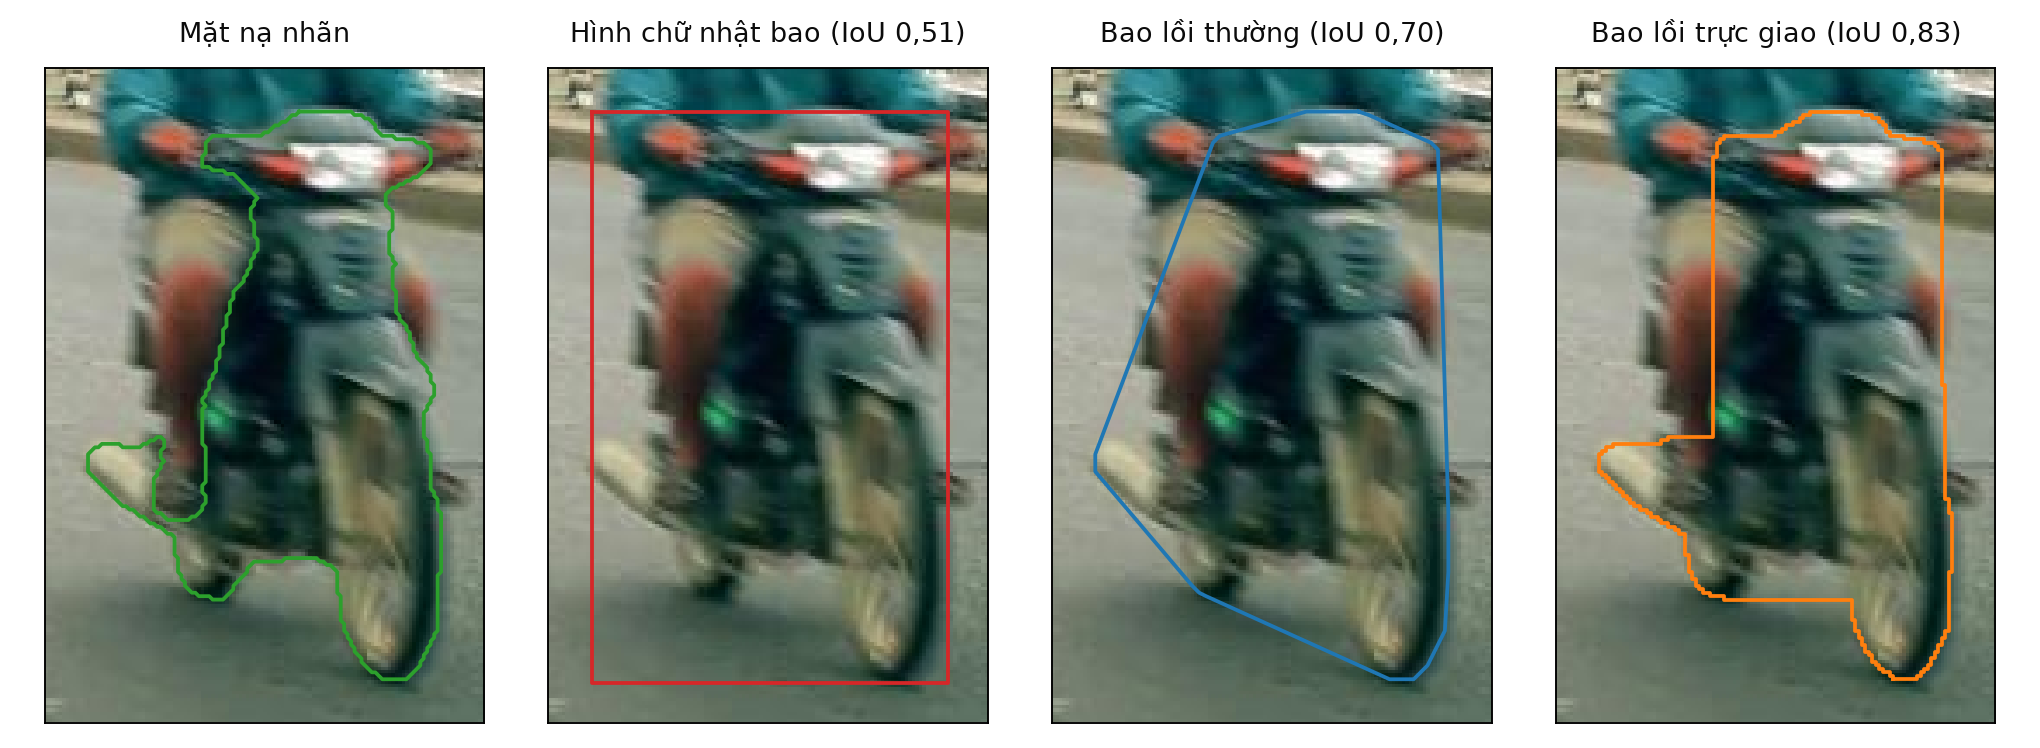
\includegraphics[width=\textwidth]{hull_real_vehicle.png}
\caption{Bốn cách biểu diễn vùng của cùng một xe máy trong bộ dữ liệu Việt Nam}
\label{fig:real_vehicle}
\end{figure}

% =====================================================================
\section{Thí nghiệm 2: Tốc độ hai bản cài đặt}
\label{sec:exp_speed}

Chỉ đo thời gian dựng bao (gồm các bước đưa đầu vào và đầu ra về cùng quy ước cho cả hai bản cài đặt) với hai bản cài đặt ở mục~\ref{sec:impl_hull}. Kết quả chỉ dùng để so sánh hai bản cài đặt của nhóm. Trung vị là giá trị ở giữa khi xếp các kết quả từ nhỏ đến lớn (nếu có hai giá trị ở giữa thì lấy trung bình của chúng). Phép đo sử dụng hai loại đầu vào:
\begin{itemize}
  \item Tổng hợp: $n \in \{100, 500, 1\,000, 2\,000, 5\,000, 10\,000\}$ điểm nguyên trong vùng $4000\times4000$,
        theo hai phân bố: \emph{đều} trong hình vuông (bao có ít đỉnh) và \emph{trên đường tròn} (hầu hết các điểm
        đều là đỉnh bao, trường hợp xấu).
  \item Đường biên thật: biên đầy đủ của 540 mặt nạ nhãn Việt Nam (12--1\,768 điểm, trung vị 165),
        mỗi xe lấy trung vị 5 lượt.
\end{itemize}

Hình~\ref{fig:synthetic_distributions} minh hoạ hai kiểu dữ liệu tổng hợp: phân bố đều là các điểm được lấy ngẫu nhiên khắp vùng vuông, còn dữ liệu đường tròn chỉ có điểm trên đường viền tròn.

\begin{figure}[H]
\centering
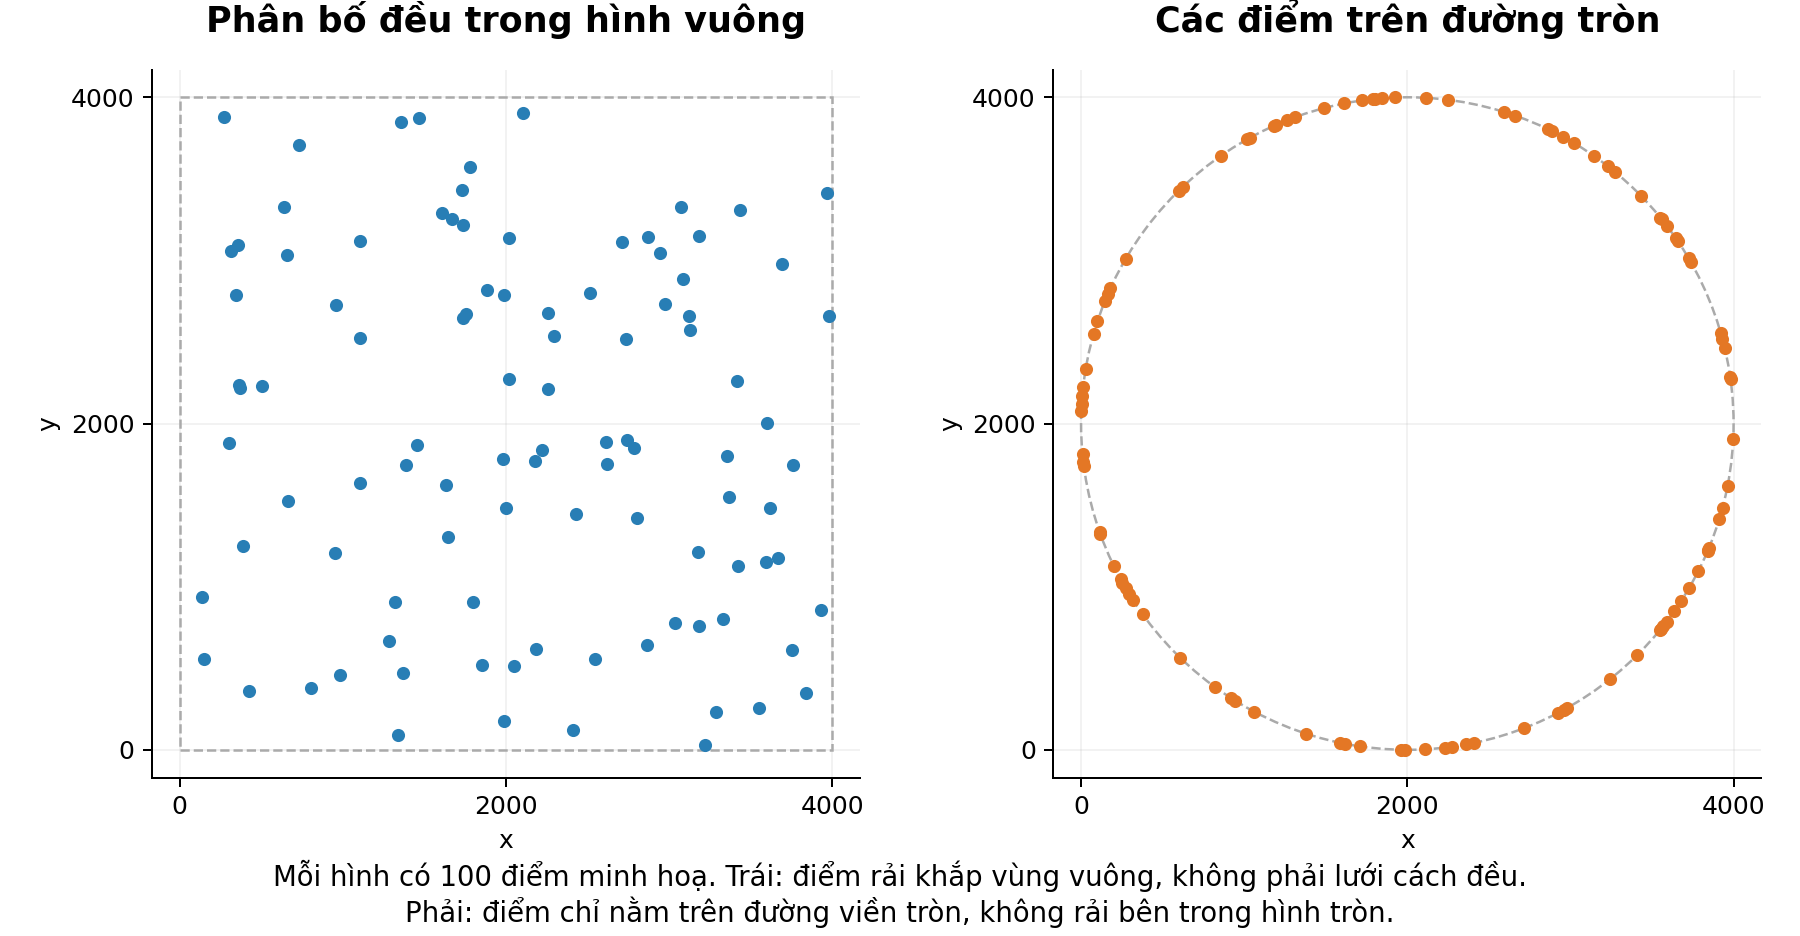
\includegraphics[width=\linewidth]{synthetic_point_distributions.png}
\caption{Hai kiểu dữ liệu dùng để đo tốc độ, minh hoạ với 100 điểm mỗi kiểu trong vùng $4000\times4000$. Trái: điểm ngẫu nhiên theo phân bố đều trong hình vuông. Phải: điểm có góc ngẫu nhiên nằm trên đường tròn, sau đó làm tròn toạ độ về số nguyên.}
\label{fig:synthetic_distributions}
\end{figure}



\begin{table}[H]
\centering
\caption{Thời gian dựng bao (ms, trung vị 30 lượt) trên tập điểm tổng hợp}
\label{tab:speed_syn}
\begin{tabular}{rrrrr}
\toprule
\multirow{2}{*}{$n$} & \multicolumn{2}{c}{Phân bố đều} & \multicolumn{2}{c}{Trên đường tròn} \\
\cmidrule(lr){2-3}\cmidrule(lr){4-5}
 & Bản QuickHull & Graham & Bản QuickHull & Graham \\
\midrule
100    & 0,27  & 0,29  & 0,65  & 0,32 \\
500    & 1,41  & 1,31  & 9,02  & 1,43 \\
1\,000 & 2,21  & 2,35  & 31,2  & 2,80 \\
2\,000 & 3,79  & 4,59  & 101,7 & 5,54 \\
5\,000 & 9,14  & 11,66 & 404,6 & 12,7 \\
10\,000& 22,5  & 25,8  & 918,9 & 22,8 \\
\bottomrule
\end{tabular}
\end{table}

\begin{table}[H]
\centering
\caption{Thời gian dựng bao trên 540 đường biên xe thật}
\label{tab:speed_real}
\begin{tabular}{lrrr}
\toprule
Bản cài đặt & Trung vị (ms) & Trung bình (ms) & Tổng 540 xe (ms) \\
\midrule
Bản QuickHull & 0,648 & 1,509 & 815 \\
Graham            & \textbf{0,458} & \textbf{0,658} & \textbf{356} \\
\bottomrule
\end{tabular}
\end{table}

\begin{figure}[H]
\centering
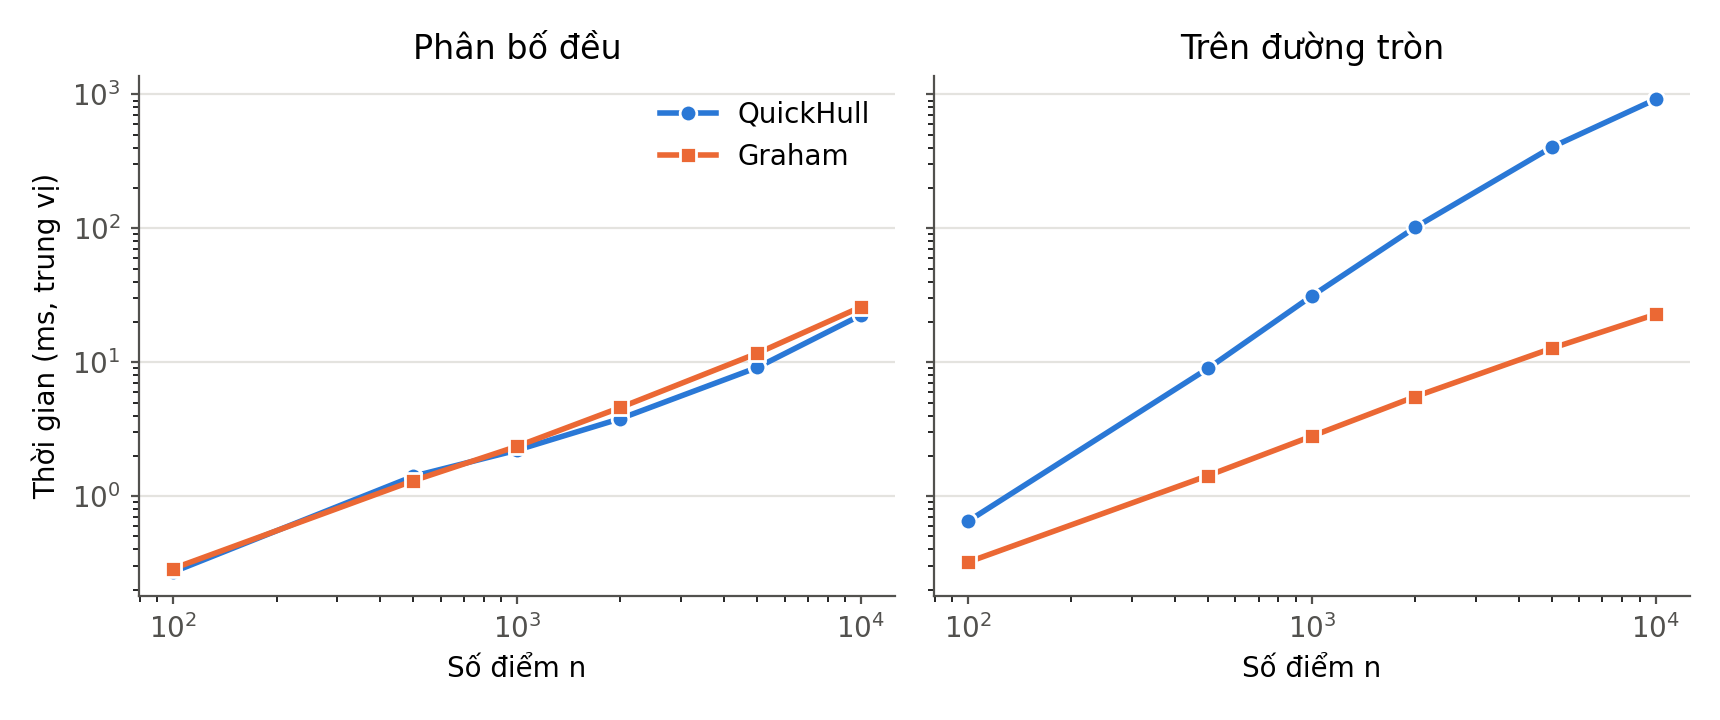
\includegraphics[width=\textwidth]{hull_speed.png}
\caption{Thời gian dựng bao theo số điểm; cả hai trục dùng thang logarit, tức các khoảng cách bằng nhau trên trục biểu diễn cùng một mức tăng theo tỉ lệ. Trái: phân bố đều; phải: trên đường tròn.}
\label{fig:speed}
\end{figure}

Từ các kết quả trên có thể rút ra:
\begin{itemize}
  \item Với phân bố đều, thời gian hai bản cài đặt gần nhau; bản QuickHull nhanh hơn một chút ở $n$ lớn.
  \item Với điểm trên đường tròn, thời gian của bản QuickHull tăng nhanh hơn nhiều so với mức tăng của số điểm, phù hợp với cận xấu nhất $O(n^2\log n)$ nêu trong Bảng~\ref{tab:algo_compare}.
        Thời gian O-Graham vẫn tăng gần theo tỉ lệ với số điểm nên nhanh hơn rõ rệt khi $n$ lớn.
  \item Trên đường biên xe thật, bản Graham có thời gian trung vị và trung bình thấp hơn bản QuickHull.
  \item Mỗi cấu hình tổng hợp dùng một tập điểm cố định, được tạo với cùng giá trị khởi tạo bộ sinh số ngẫu nhiên (hạt giống), nên 30 lượt đo phản ánh biến thiên thời gian trên đầu vào đó, không phải trên nhiều tập điểm.
  \item Hai bản QuickHull và Graham cho cùng vùng bao trên các cấu hình đã thử.
\end{itemize}

% =====================================================================
\section{Thí nghiệm 3: Thay mặt nạ YOLO bằng bao lồi trực giao}
\label{sec:exp_quality}

Thí nghiệm này dùng YOLO11-l trên bộ Việt Nam, so bốn cách biểu diễn vùng cùng lấy từ một dự đoán: hình chữ nhật, bao lồi thường, bao trực giao và mặt nạ.
Bao được dựng từ chính mặt nạ, nên phép so cho biết việc đơn giản hoá mặt nạ thành bao làm mất bao nhiêu độ khớp với nhãn và đổi lại được gì.
Bao không sửa được xe bị bỏ sót hay sai lớp.

\subsection{Mức giảm chất lượng}

\begin{figure}[H]
\centering
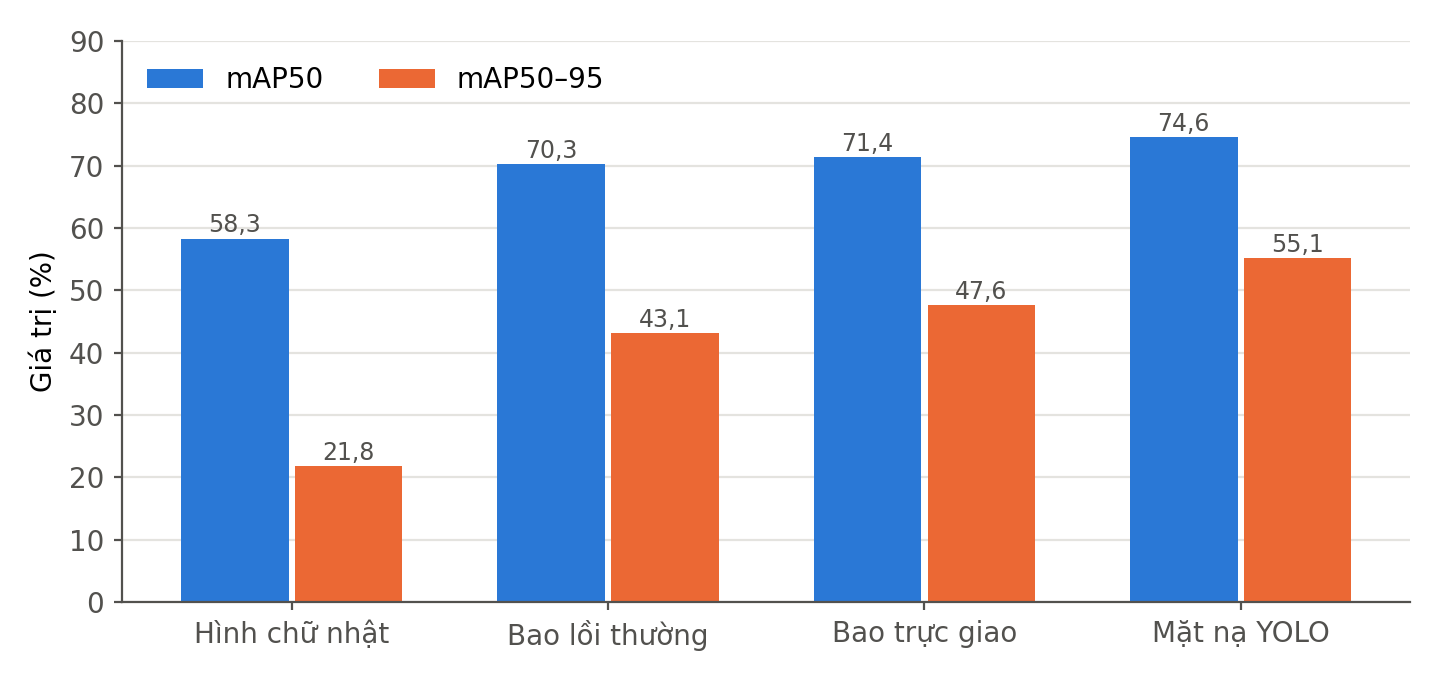
\includegraphics[width=0.85\textwidth]{mask_vs_hull_map.png}
\caption{mAP50 và mAP50--95 của bốn cách biểu diễn vùng (YOLO11-l, bộ Việt Nam; ghép đúng lớp, so với cùng mặt nạ nhãn)}
\label{fig:mask_vs_hull}
\end{figure}

\begin{table}[H]
\centering
\caption{Kết quả trên 100 ảnh Việt Nam, mô hình YOLO11-l (540 nhãn)}
\label{tab:vn_large}
\begin{tabular}{lrrrrr}
\toprule
Đầu ra & Precision & Recall & F1 & mAP50 & mAP50--95 \\
\midrule
Hộp phát hiện & 73,1\% & 70,0\% & 71,5\% & 72,3\% & 56,0\% \\
Vùng hình chữ nhật   & 61,3\% & 58,7\% & 60,0\% & 58,3\% & 21,8\% \\
Bao lồi thường        & 71,0\% & 68,0\% & 69,4\% & 70,3\% & 43,1\% \\
Bao trực giao        & 72,1\% & 69,1\% & 70,6\% & 71,4\% & 47,6\% \\
Mặt nạ YOLO     & 74,9\% & 71,7\% & 73,2\% & 74,6\% & 55,1\% \\
\bottomrule
\end{tabular}
\end{table}

Ý nghĩa các chỉ số được giải thích ở mục~\ref{sec:metrics}. Hàng Hộp phát hiện so hộp với hộp nhãn nên là một phép đo khác, không so trực tiếp được với bốn hàng vùng điểm ảnh.
Hai bản cài đặt bao trực giao cho kết quả trùng nhau ở mọi độ đo. Từ các kết quả này:
\begin{itemize}
  \item So với mặt nạ YOLO, bao giảm nhẹ ở mAP50 và giảm nhiều hơn ở mAP50--95. Nguyên nhân là bao lấp thêm các phần lõm của mặt nạ:
        xe vẫn được nhận ra, nhưng vùng không còn khớp sát như mặt nạ.
  \item So với vùng hình chữ nhật, bao tốt hơn rõ rệt, nhất là ở mAP50--95.
  \item So với bao lồi thường, bao cao hơn nhẹ ở mAP50 và cao hơn rõ hơn ở mAP50--95. Như vậy, kết quả của CH1 cũng đúng trên mặt nạ dự đoán.
\end{itemize}

Mức giảm mAP50--95 từ mặt nạ xuống bao có ở cả bốn lớp xe, không chỉ xe máy, và lớn hơn ở bus (chỉ 26 nhãn) và motorcycle.

\subsection{Ma trận nhầm lẫn}

Ghép không xét lớp cho thấy trong các cặp đã định vị được, YOLO11-l phân loại đúng 92,7\%.
Lỗi nhiều nhất là car $\rightarrow$ truck (12 trường hợp), tiếp theo là truck $\rightarrow$ car (9) và
truck $\rightarrow$ bus (8). Xem trực quan các ca car $\rightarrow$ truck thì chủ yếu là
xe van và xe gầm cao; các ca truck $\rightarrow$ bus chủ yếu là xe tải thùng cao phủ bạt.

\begin{figure}[H]
\centering
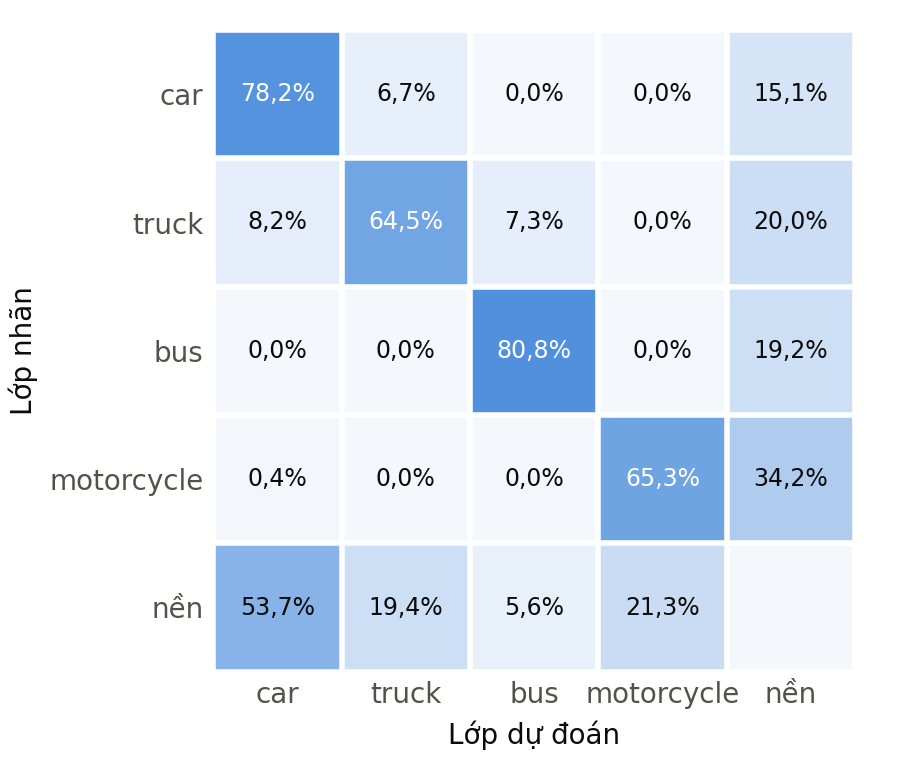
\includegraphics[width=0.62\textwidth]{vn_large_confusion.png}
\caption{Ma trận nhầm lẫn của mặt nạ YOLO (YOLO11-l), chuẩn hoá theo hàng. Hàng ``nền'' là phân bố các dự đoán thừa theo lớp.
}
\label{fig:vn_class}
\end{figure}

\subsection{Độ gọn và tính liên thông của vùng bao}

So với đường biên đã được OpenCV rút gọn, số đỉnh của bao chỉ ít hơn một phần nhỏ, nên độ gọn không phải lợi ích chính.
Lợi ích rõ hơn là về hình học: bao luôn là một vùng liền khối, không lỗ, các cạnh song song với trục, nên diện tích và chu vi tính trực tiếp từ đỉnh,
trong khi khoảng một phần năm mặt nạ bị đứt thành nhiều mảnh. Nối các mảnh cũng có thể làm bao lấp sang vùng không phải xe, như ca giảm nhiều nhất ở Hình~\ref{fig:crops}.

\begin{figure}[H]
\centering
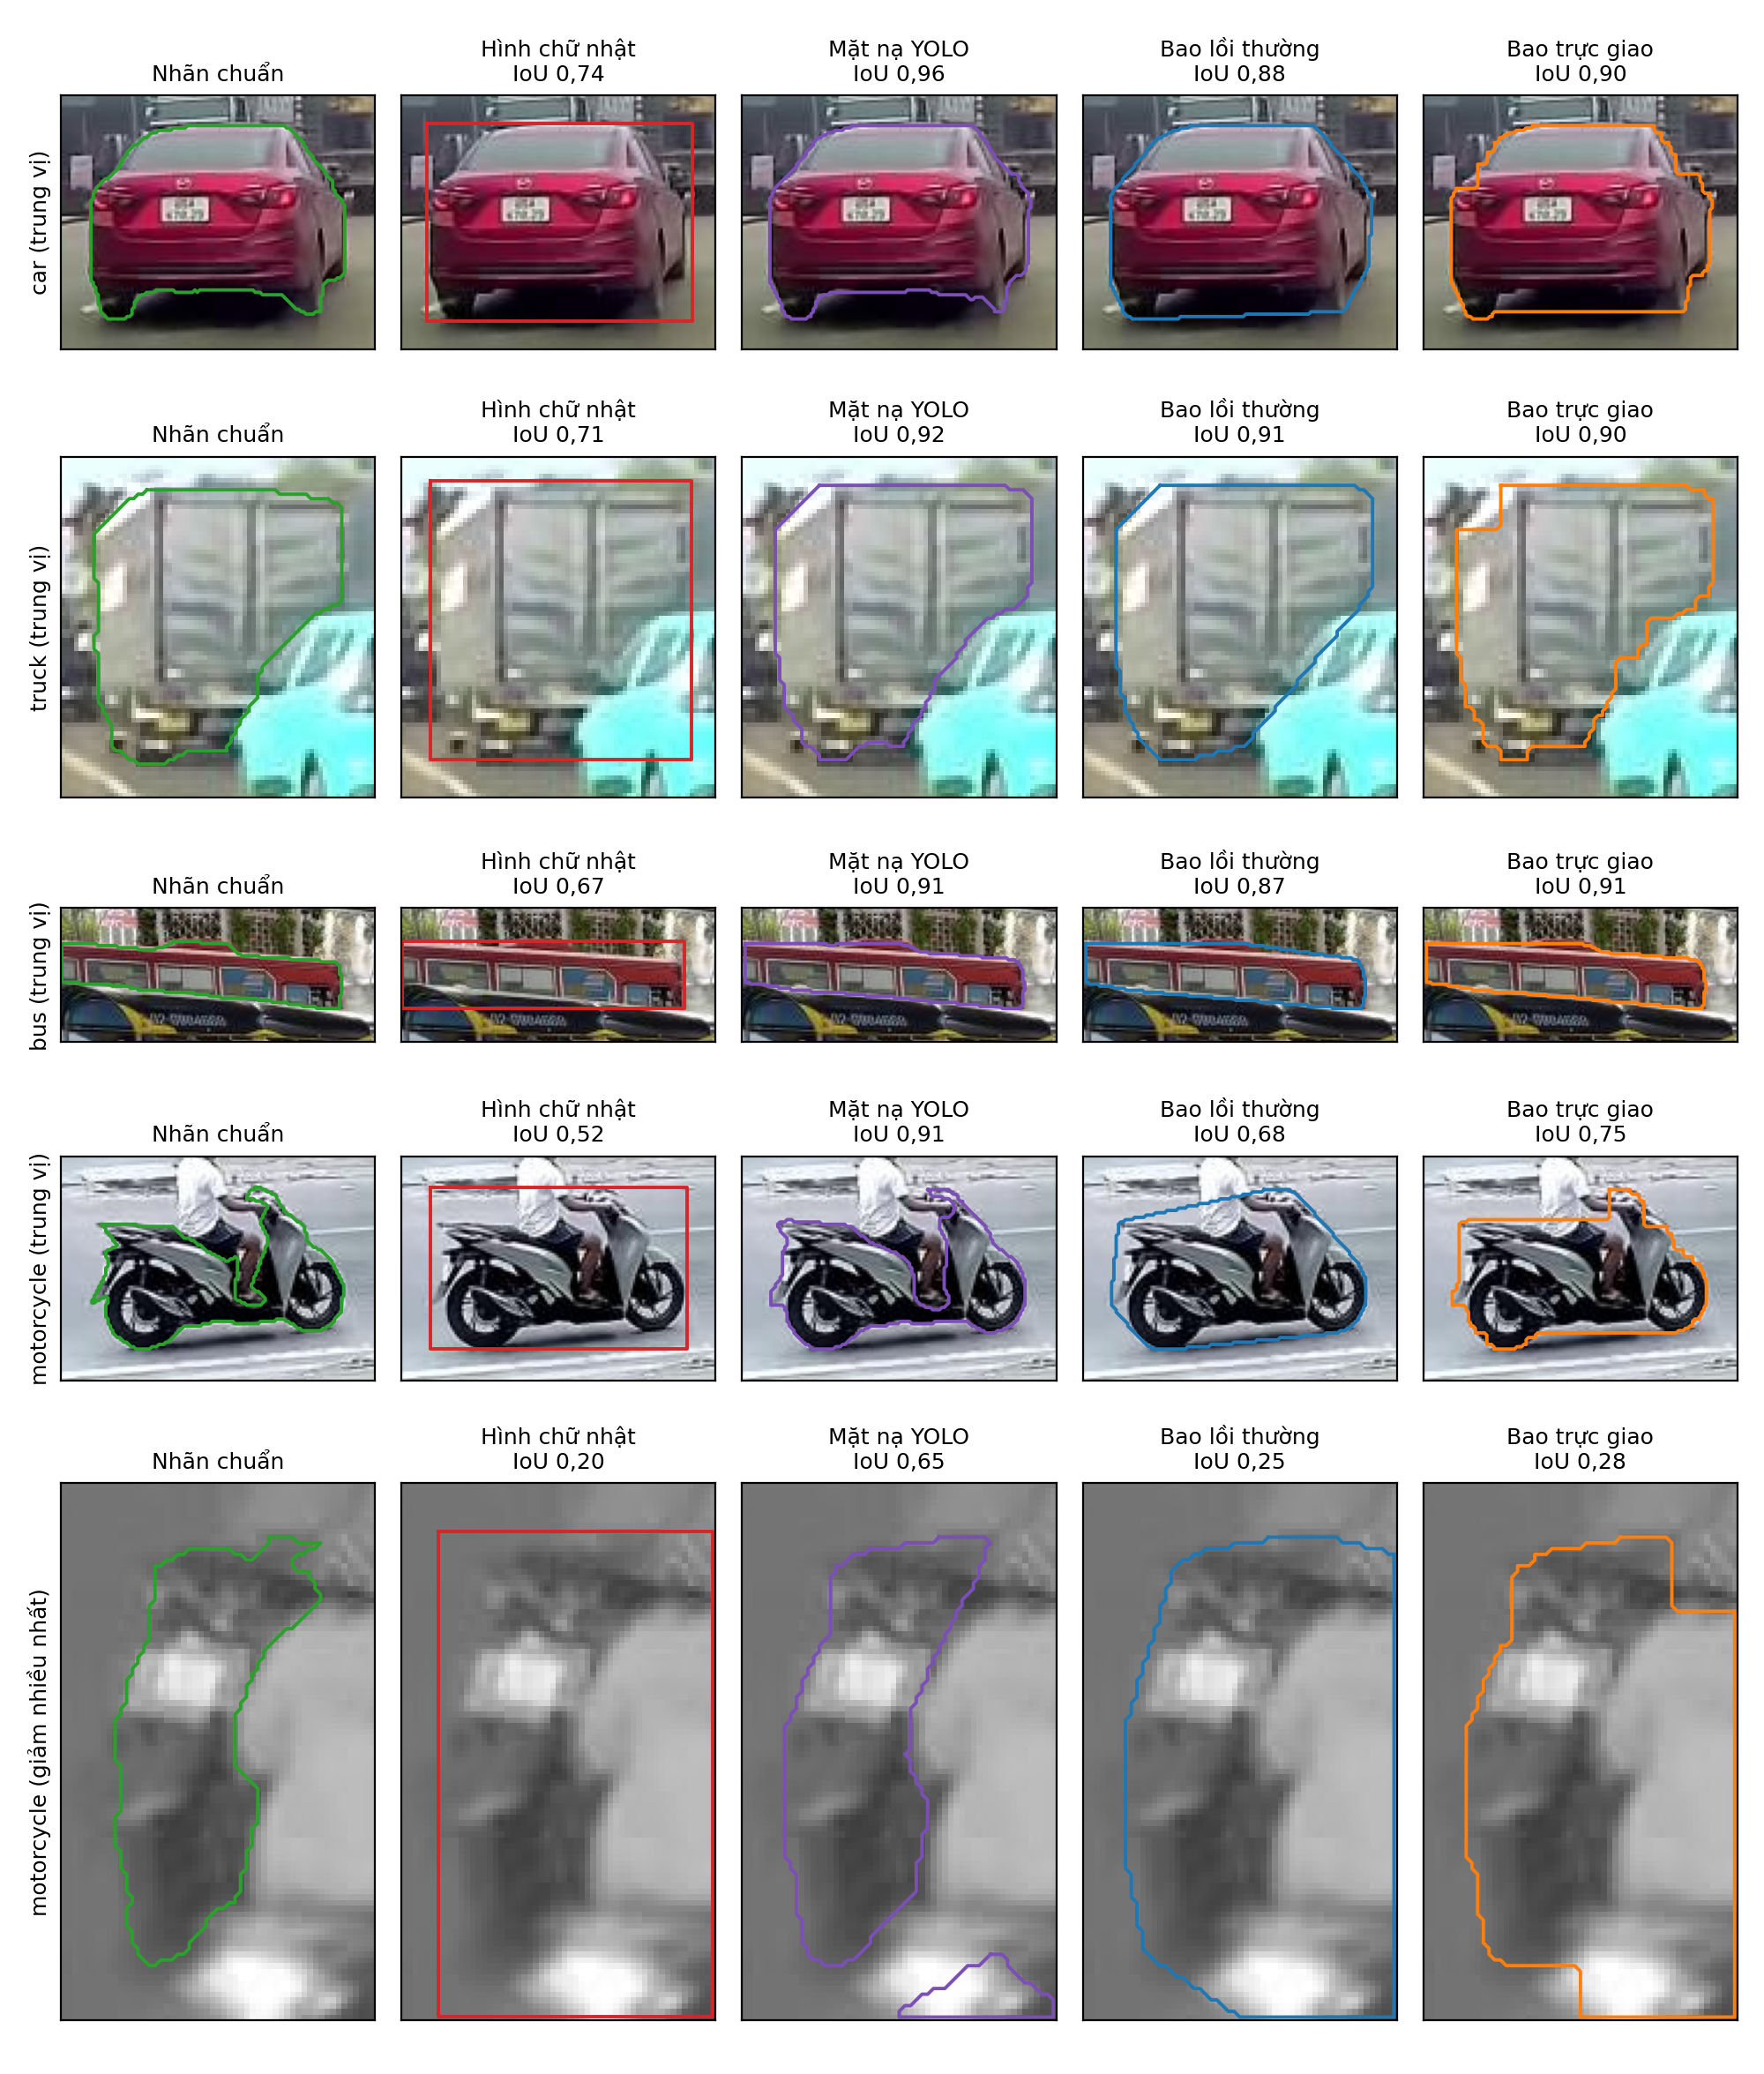
\includegraphics[width=\textwidth]{crop_compare.png}
\caption{Cùng một xe và cùng khung cắt, YOLO11-l trên bộ Việt Nam; IoU so với cùng nhãn. Chọn từ 219 cặp ghép đúng có nhãn từ 1\,600 điểm ảnh trở lên:
bốn hàng đầu là xe có IoU bao trực giao ở trung vị của từng lớp, hàng cuối là ca bao giảm IoU nhiều nhất so với mặt nạ. Đây là ví dụ minh hoạ, không đại diện cho xe nhỏ.}
\label{fig:crops}
\end{figure}

% =====================================================================
\section{Kết quả định tính}
\label{sec:qualitative}

Hình~\ref{fig:scenes} chọn ảnh theo F1 của mặt nạ YOLO trên bộ Việt Nam. Mỗi hàng gồm nhãn chuẩn (xanh dương), mặt nạ YOLO và bao trực giao.
Màu xanh lá là dự đoán đúng (TP), đỏ là dự đoán sai (FP), cam là nhãn bị bỏ sót.

\begin{figure}[H]
\centering
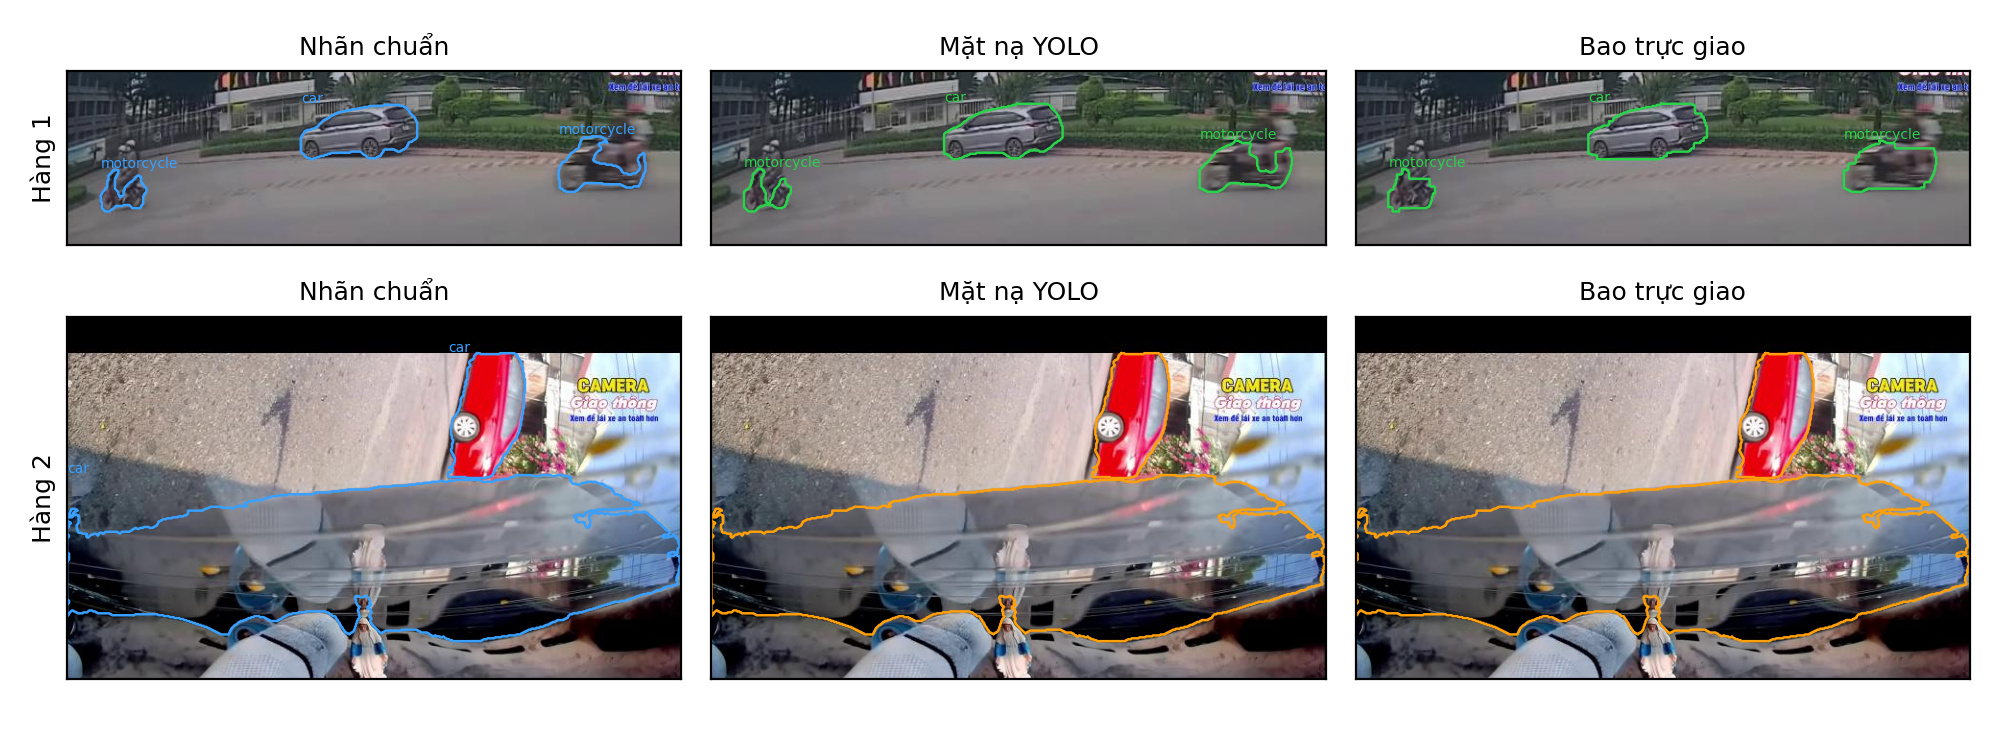
\includegraphics[width=\textwidth]{scene_compare.png}
\caption{YOLO11-l, bộ Việt Nam, độ tin cậy $\ge 0{,}20$. Hàng 1: ảnh dễ có F1 cao nhất. Hàng 2: ảnh khó có F1 thấp nhất, gồm một nhãn \texttt{car} đặt nhầm lên táp-lô
và một xe ở mép ảnh bị cắt, mô hình không phát hiện được.}
\label{fig:scenes}
\end{figure}

\paragraph{Minh hoạ trên video.}
Hệ thống dùng YOLO11-l kết hợp ByteTrack có sẵn trong Ultralytics để gắn ID, rồi dựng bao cho các xe có ID và mặt nạ. Hình~\ref{fig:video} được chọn ở khoảng giây thứ 5,2 của video ban đêm, sau khi xử lý một đoạn liên tiếp 36 khung hình bằng YOLO11-l và ByteTrack; bao được vẽ bằng bản Graham. Đây là minh hoạ chức năng, không phải phép đánh giá độ chính xác theo vết hay tốc độ toàn hệ thống; video không có nhãn ID chuẩn.

\begin{figure}[H]
\centering
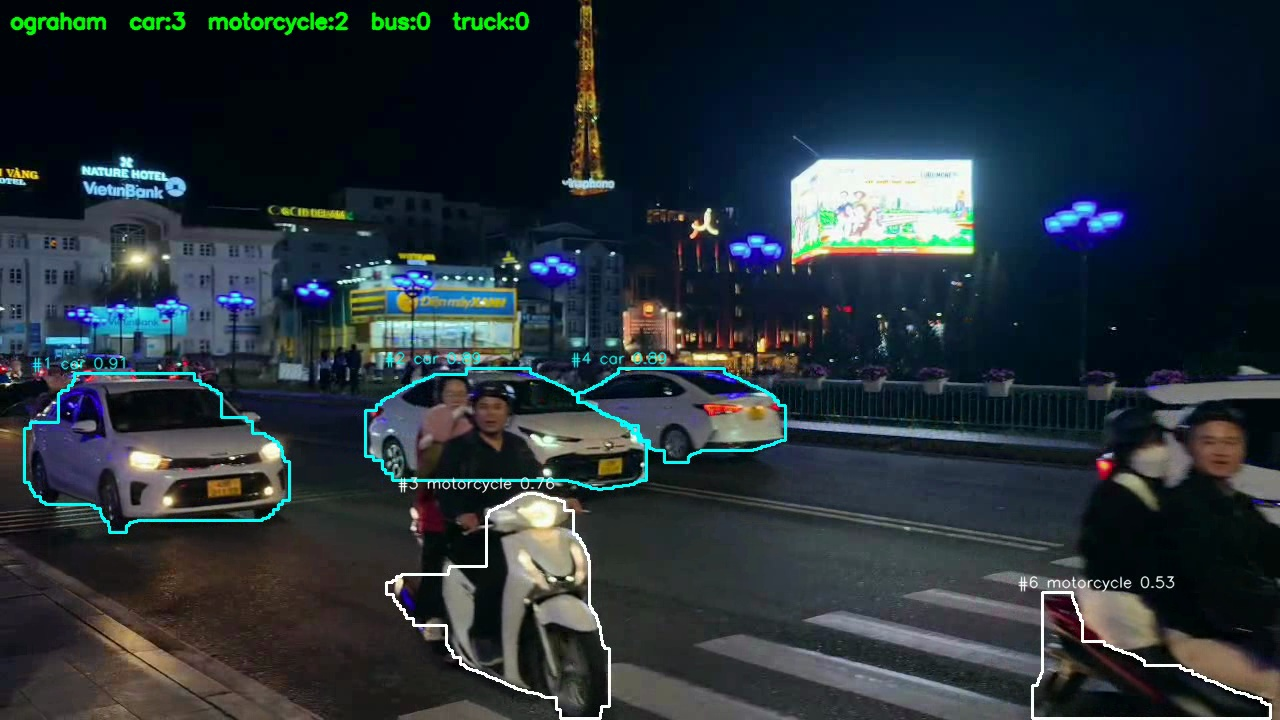
\includegraphics[width=\textwidth]{video_preview_night.jpg}
\caption{Đầu ra YOLO11-l kết hợp ByteTrack trên video giao thông ban đêm do nhóm cung cấp; bao được vẽ bằng bản Graham. Mỗi xe được hiển thị ID, lớp, độ tin cậy và vùng bao. Các số đếm ở góc trên là số đối tượng đang được hiển thị trong khung hình, không phải tổng số xe đi qua.}
\label{fig:video}
\end{figure}

% =====================================================================
\section{Thảo luận}
\label{sec:discussion}

\paragraph{Lựa chọn bản cài đặt.} Hai bản cài đặt cho cùng một bao trên dữ liệu thử, nên lựa chọn dựa trên tốc độ. Trong hai bản được khảo sát,
nhóm chọn O-Graham vì nhanh hơn trên đường biên xe và không chậm đi khi bao nhiều đỉnh. Đây là so sánh giữa hai bản cài đặt của nhóm,
không phải kết luận về O-Quickhull gốc: bài báo~\cite{nguyen2022quickhull} cho thấy O-Quickhull nhanh hơn O-Graham trên phần lớn dữ liệu họ thử.

\paragraph{Phạm vi sử dụng bao lồi trực giao.} Mặt nạ YOLO vẫn khớp nhãn tốt nhất ở mức điểm ảnh.
Bao lồi trực giao phù hợp khi cần một vùng \emph{liên thông, không lỗ}, có diện tích và chu vi tính trực tiếp, và sát nhãn hơn hình chữ nhật và bao lồi thường.
Các ứng dụng như ước lượng diện tích mặt đường bị chiếm hay kiểm tra va chạm vùng giữa các xe là hướng có thể dùng, nhưng chưa được đánh giá trong đồ án.

\paragraph{Giới hạn của đánh giá.}
\begin{itemize}
  \item Bộ 100 ảnh Việt Nam được chọn có chủ đích (70\% ảnh dễ), nhiều ảnh trích từ cùng một video nên có tương quan;
        kết quả không đại diện ngẫu nhiên cho giao thông Việt Nam.
  \item Nhóm đã thử fine-tune trên dữ liệu Việt Nam nhưng chưa ghi nhận cải thiện; các kết quả trong chương này sử dụng mô hình huấn luyện sẵn.
  \item Chưa khảo sát ảnh hưởng của kích thước đầu vào: ảnh $640\times640$ được phóng lên \texttt{imgsz=960} khi inference.
  \item Nhãn còn một số lỗi chưa sửa, được phát hiện khi xem trực quan: bộ Việt Nam có 7 xe van gán \texttt{car},
        khoảng 34 polygon nghi chỉ phủ một phần xe (22 ca là xe máy) và 4 nhãn đặt nhầm lên táp-lô hoặc gương xe. Polygon thiếu làm giảm recall xe máy:
        tính theo hộp, YOLO11-l đạt 61,8\% ở ngưỡng IoU 0,5 và 68,9\% ở ngưỡng 0,3.
\end{itemize}
